A widely used surface sensitive method is the scanning tunneling microscopy (STM). \index{STM} It is used to investigate as well the topography of the sample, as its electronic configuration by utilizing the quantum mechanical tunneling effect. 

Because a wave function of a electron does not strictly end within the sample, parts of the electronic wave function spill unto the surrounding vacuum. If another material (STM tip) is in close proximity, electrons can overcome the vacuum barrier and cross the vacuum gap into the other material - a process known as tunneling.  Assuming the two materials are the same, the created, time averaged current is zero because the same amount of electrons tunnel in either direction. If a voltage is applied across the vacuum gap, the current in one direction becomes non-zero. This voltage - called bias - may be changed and switched in polarity, causing electrons to originate from either the tip or the sample. This enables detection of either occupied (negative bias) or unoccupied (positive bias) states in the sample. The distance between tip and sample influences the amount of electrons that are able to tunnel and gives rise to the resolution of geometric details in STM images. With a constant bias the current is related to the distance between tip and the (homogeneous) sample.

The position of the tip (x, y, z) is controlled with a set of piezos (see figure \ref{fig:STM-tip}). In this work a tubular piezo stack is used to control the tips position with a central piezo element located on top of the tungsten tip. The piezo length can be controlled with the voltage applied to them, which is used to choose not only the tip-sample distance, but other parameters like image size and scan speed as well. All of these parameters are monitored with the STM software. A feedback loop controls the piezo voltages. For recording an image the area is raster scanned in consecutive lines, applying a sawtooth voltage to the fast scan direction along the line. The next lines are chosen by slowly increasing the voltage along the slow scan direction. Depending on the operating mode the tip-sample distance is controlled by piezo elements, too.

%\begin{figure}[ht]
%	\begin{center}
%	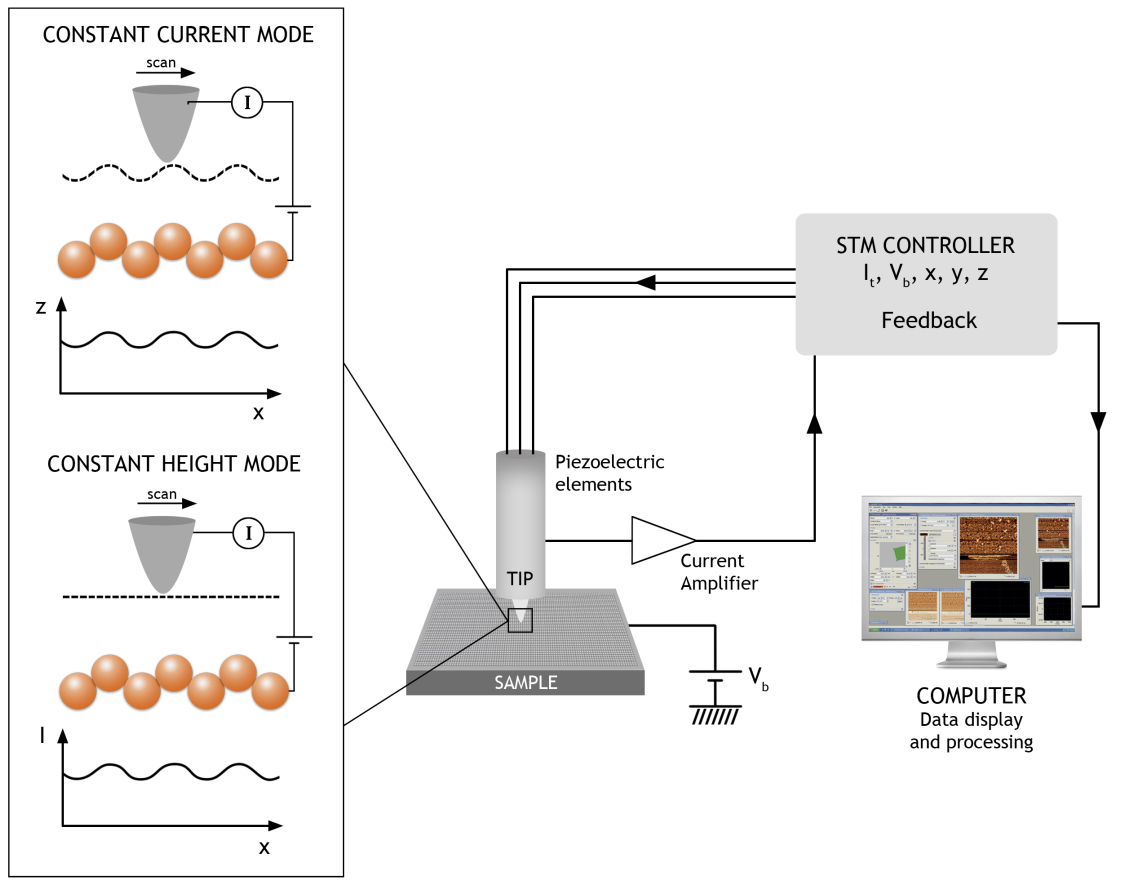
\includegraphics[width=0.45\textwidth]{./images/STM-sketch.jpg}
%	\end{center}
%	\caption{Taken from \cite{diss-manuela}}
%
%\end{figure}

\begin{figure}\centering
	\subfigure[Macroscopic view on the STM tunnel junction. The main piezo is divided in four parts to control movement in the x-y plane and tip-sample distance. Adopted from \cite{STM-rutgers}]{\includegraphics[width=0.6\textwidth]{./images/STM-rutgers-modified}\label{fig:STM-tip}}
	\subfigure[From \cite{diss-manuela}]{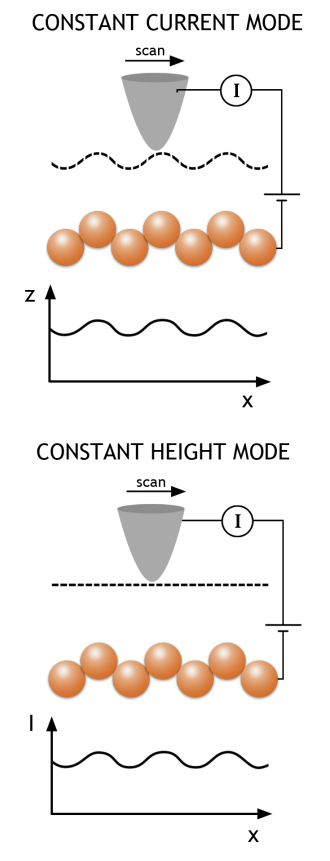
\includegraphics[height=0.3\textwidth]{./images/STM-sketch-cut.jpg}\label{fig:STM-modes}}
	\caption{Operating principles of an STM. A macroscopic sketch \ref{fig:STM-tip} shows the central piezo that controls the tip position above the sample. A microscopic sketch shows the tips movement in constant current mode while moving across a atomic step edge. The difference between constant current and constant height mode is shown in \ref{fig:STM-modes}. While the tip follows the samples LDOS in constant current mode (top) the tip height remains constant in constant height mode (bottom).}
	\label{fig:STM-sketch}
\end{figure}

There are two common ways to operate an STM as shown in figure \ref{fig:STM-modes}.
The \textbf{constant current mode}\index{STM:operating mode} is the most widely used one. The tip height is regulated with a feedback controller to achieve a constant tunneling current for the chosen bias. The recorded information is now the voltage applied to the z-piezo to maintain a plane with the same current.
In \textbf{constant height mode} the tip has always the same absolute height (no feedback control), but as the tip-sample distance changes the tunneling current varies, which then is the measured quantity.
To avoid crashes when the sample is very irregular, many STM's are operated in constant current mode. Typical tunneling currents are in the range of \SIrange{0.01}{100}{\nA} where the applied voltage may range from \SIrange{0.01}{10}{\volt}. All STM images in this work are recorded in constant current mode.
The current recorded in a certain area of the sample is translated into a contrast variation on a color scale. While some images encourage the operator to interpret points with high intensity as elevated atoms it is not that trivial. Tunneling current between tip and sample depends on the LDOS of tip and surface and is therefore not implicitly maximized at the atomic positions. It may also vary with the bias voltage applied in a non-trivial manner. Investigation of this behavior led to the establishment of a new measurement technique, called scanning tunneling spectroscopy (see section \ref{section:STS}). 

``This results in a non zero tunneling current when the tip is in the lateral neighborhood of the adsorbate. This contributes to the apparent expansion of the adsorbate print in its STM image compared to the position of its atoms. Interferences between through-adsorbate and through-space tunneling processes participate to this effect which depends on orbital-symmetry and tip-shape. A local density of states calculation [8,14,28] is not adapted to grasp this effect since he tip is considered far away from the surface. Moreover, in such calculations, the tip radius or the tip-substrate distance is generally optimized to fit the lateral size of the adsorbate print with the experimental image [8,28].''\cite{sautet_interpretation_1992}.

\index{STM!One dimensional tunneling}
Most information in here refers to \cite{bonnell_scanning_1993}.
While the tip (metal) is far away from the sample, their vacuum levels are supposed to be the same. The corresponding Fermi energies of sample and tip lie below the vacuum level by the amount of their work functions ($\Phi_s$ and $\Phi_t$ for sample and tip respectively). Wave functions of electrons within the solids decay exponentially in vacuum, depended on their energy with respect to the Fermi level.
If sample and tip are in thermodynamic equilibrium, their Fermi levels are the same. Electrons now face a potential barrier (approximately rectangular) which can be overcome if their energy is high enough and the barrier sufficiently narrow. When a voltage is applied across the tunneling barrier, the energy of the tip-electrons is shifted by $eV$. When a positive bias voltage is applied, electrons tunnel from the tip into unoccupied states in the sample - a negative bias results in a tunneling current in opposite direction. Since states with highest energy have the largest decay lengths in vacuum, most of the tunneling current is determined by electrons within close proximity to the Fermi level.

\begin{figure}[ht]
	\begin{center}
	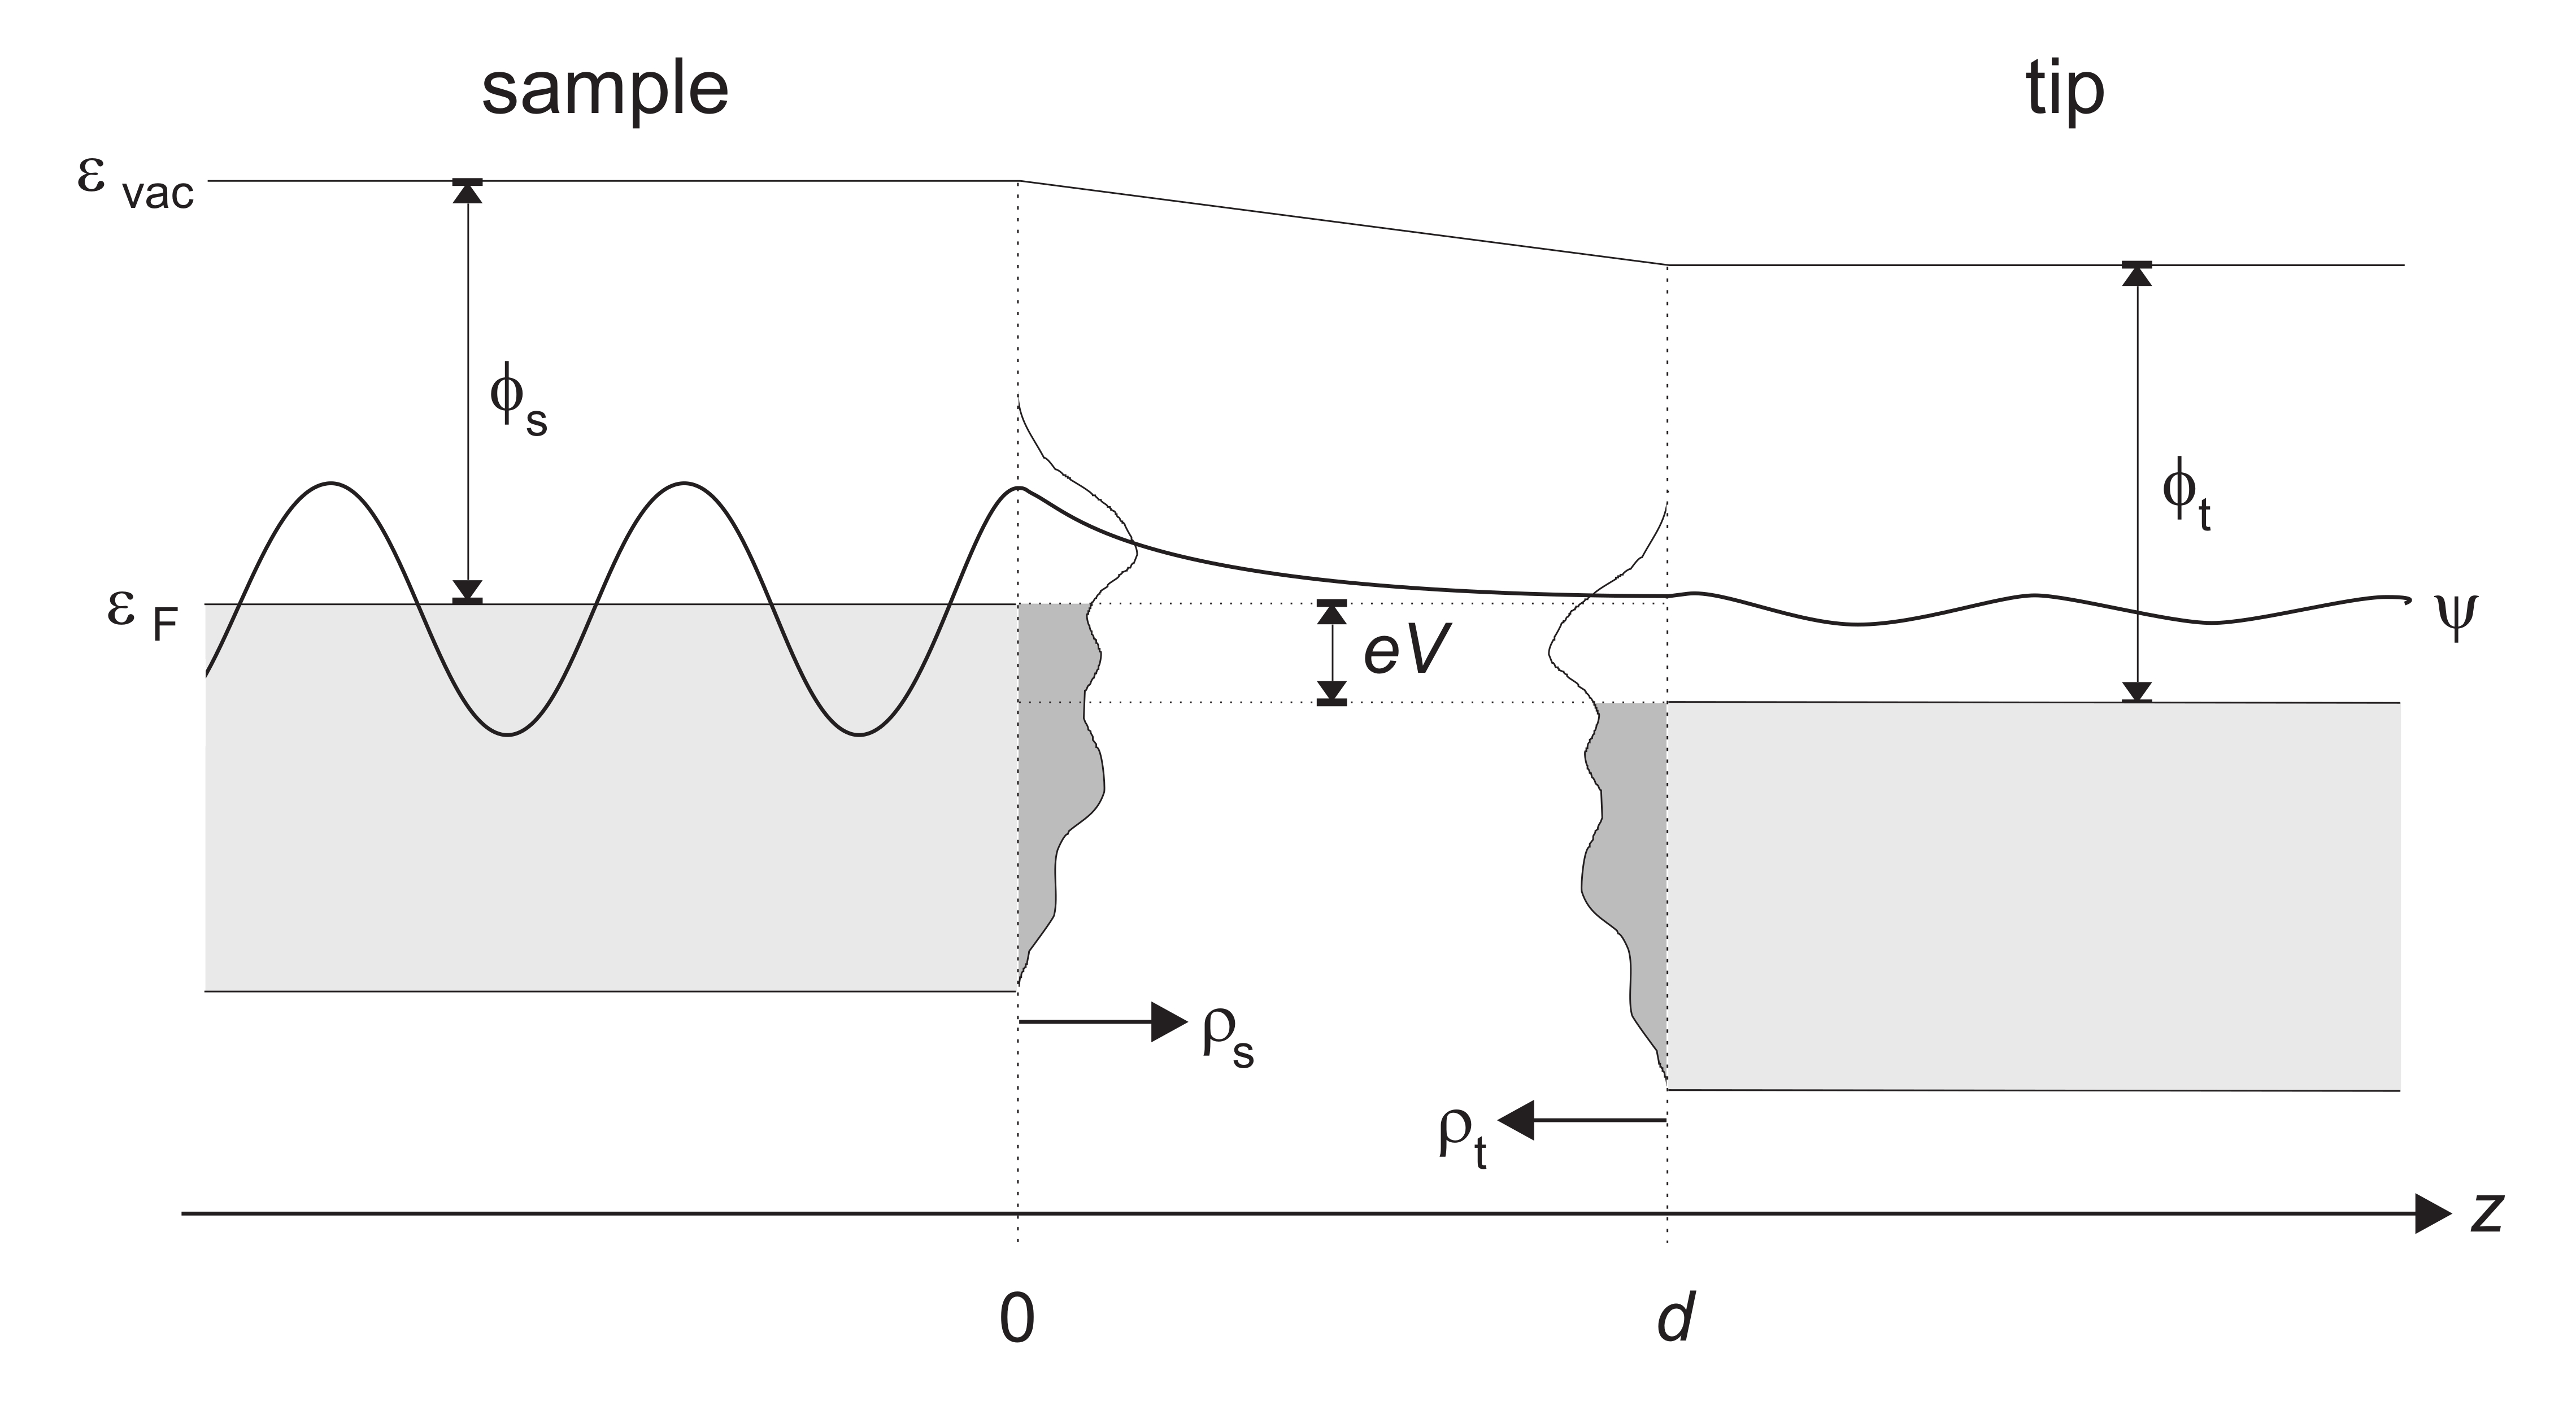
\includegraphics[width=0.45\textwidth]{./images/tunnel-barrier.jpg}
	\end{center}
	\caption{Taken from \cite{diss-schunack}}
\end{figure}


The tunneling current at a given distance is determined by:
\begin{itemize}
 \item The applied voltage
 \item The density of states of electron source and destination
\end{itemize}

Following the model of \index{STM!Tersoff-Hamann} Tersoff-Hamann\footnote{Please note that there are more models and corrections to them. An evolution from Bardeen's approach to the one done by Tersoff-Hamann can be found here \cite{lounis_theory_2014} including Chen’s expansion.}((1) uniform density of states in the tip, (2) temperature is low, (3) small bias voltage of some mV, (4) waveform of electrons in tip are s-waves) the tunneling current results to 
$$I=32\pi^3\hbar^{-1}e^2V\Phi^2 R^2\kappa^{-4}e^{2\pi R}D_1(E_F)\rho(r_o,E_F)$$ where $D_1$ is the density of states per unit volume of the tip, R the tip radius and $\rho(r_0,E_F)$ the Fermi level density of states in the sample. If I is held constant one can see that the tip in principle follows a contour of constant Fermi level density of states, measured at the center of the curvature of the s-wave like tip. While its a good first approximation of the system, in many cases the bias is much higher than 10mV (\SIrange{1}{5}{\V}) more than just the electrons near Fermi contribute.

Using \index{STM!WKB} WKB theory the tunneling current is given by
\begin{equation}
I=\int_0^{eV}\rho_s(r,E)\rho_t(r,eV+E)T(E,eV,r)dE
\label{WKB}
\end{equation}
where $\rho_s(\rho_t)$ is the density of states of the sample (tip) and T is the tunneling transmission probability
\begin{equation}
T(E,eV)=exp\left(-\frac{2Z\sqrt{2m}}{\hbar}\sqrt{\frac{\Phi_s+\Phi_t}{2}+\frac{eV}{2}-E}\right)
\label{Transmission-function} 
\end{equation}
If $eV<0$ the tunneling current is largest for $E=0$ (electrons on the Fermi-level of the sample), if $eV>0$ the tunneling current is largest for $E=eV$ (electrons of Fermi level in tip).

Due to the fact that the tunneling current is proportional the density of states in the tip AND the molecule one can deduce the band structure within a range of several volts in the vicinity of the Fermi energy.

This is in line with the assumption that waves of electrons decay exponentially, the most energetic electrons having the largest decay length.

\index{STM:resolution}The accuracy of a STM is very high with spatial resolution down to the atomic scale. Due to the fact that the tips motion is controlled with different piezos, one has to take different elongations in different directions into account. For example, if the STM scans the fast scanning direction just a bit further than the slow scan direction, the resulting image (although pixel wise square) is no longer physically square anymore. Imagine a square (1:1 side ratio, diagonal angle 45\textdegree) where one side is elongated in the image by 5\%. The resulting square (1:1.05 side ratio, diagonal angle 43.6\textdegree) looks square because it has the equal number of pixels in both directions, but it is physically rectangular. The expression used to calculate the uncertainty with known calibration parameters is
$$\Delta \Theta = 45 - \frac{180}{\pi}\cdot\arctan(\frac{1}{1+x})$$ where x is the percentage of one side being longer. This results in an uncertainty of 0.3\textdegree(1\%), 1.4\textdegree(5\%, see example above), 2.7\textdegree(10\%). For moderate shear, conformity is almost conserved and the uncertainty below 2\textdegree.

STM has a big advantage compared to space averaging, surface sensitive techniques like XPS and LEED because it offers information in the  order of atomic radii. With the help of STM the reconstructed surface of Si(111) was first discovered \cite{binnig_1983} and described on the atomic scale.